\chapter{Rest of Event Clean-up}
\label{sec:roe}

Continuing from Section \ref{sec:loose-neutrino-reconstruction}, the description of the ROE clean-up process is described here. 

Training the MVA classifiers follows the same recipe for all the steps in this chapter. For each step, we run $B$ meson reconstruction on Signal MC with a generic companion $B$ meson. This way the produced weight files are less likely to be signal-side dependent and can be used also for untagged analyses of other decays. For every correctly reconstructed signal $B$ meson we save the necessary information for each MVA step (i.e. properties of ROE clusters). Only correctly reconstructed $B$ candidates are chosen here, to prevent leaks of information from the signal side to the ROE side.

More information about the MVA training, hyper-parameter optimization and feature importance for each MVA step in this chapter can be found in Appendix \ref{sec:roe-control-plots}.

\section{Clusters Clean-up}

Photons originate from the IP region, travel to the ECL part of the detector in a straight line and produce a cluster. The direction of the photon is determined via the location of the cluster hit in the ECL and the energy of the photon is directly measured via the deposited energy. This way the four-momentum of photons is determined and used in Eq. (\ref{eq:ROEloop}).

Most of the photons in events with $B$ mesons come from processes such as $\pi^0 \to \gamma \gamma$ decays which are interesting for physics. However, a lot of hits in the ECL are also created by photons coming from the beam-induced background or secondary interactions with the detector material, which we are usually not interested in, except in cases involving material studies. Photons of the first kind should be taken into account when calculating the missing 4-momentum, while photons, which are not directly related to the collision, add extra energy and momentum to the event, which spoils our measured quantities. In the first step of the clusters clean-up, we train an MVA which recognizes good $\pi^0$ candidates and apply this information to the daughter photons. This represents a sort of a $\pi^0$ origin probability, which peaks at or is equal to 0 for photons not coming from $\pi^0$ particles, and peaks at 1 otherwise. This information is used as an additional classifier variable in the next step of the clean-up, where we train to recognize good photons in an event.

\subsection{\texorpdfstring{$\pi^0$}{π0} MVA Training}

The training dataset of $\pi^0$ candidates contains
\begin{itemize}
	\item 183255 target candidates,
	\item 200000 background candidates,
\end{itemize}
where the definition of a target is that both photon daughters that were used in the reconstruction of the $\pi^0$ are actual photons and real daughters of the $\pi^0$ particle. We use $\pi^0$ candidates from the converted Belle particle list and select those with invariant mass in the range of $M \in [0.10,~0.16]\e{GeV}$. After that we perform a mass-constrained fit on all candidates, keeping only the ones for which the fit converged. 

The input variables used in this MVA are
\begin{itemize}
	\item $p$ and $p_{CMS}$ of $\pi^0$ and $\gamma$ daughters,
	\item fit prob. of the mass-constrained fit, invariant mass and significance of mass before and after the fit,
	\item angle between the photon daughters in the CMS frame,
	\item cluster quantities for each daughter photon
	\begin{itemize}
		\item $E_9/E_{25}$,
		\item theta angle,
		\item number of hit cells in the ECL,
		\item highest energy in cell,
		\item energy error,
		\item distance to closest track at ECL radius.
	\end{itemize}
\end{itemize}

The classifier output variable is shown in Figure \ref{fig:ROE_pi0}.

\begin{figure}[H]
	\centering
	\captionsetup{width=0.8\linewidth}
	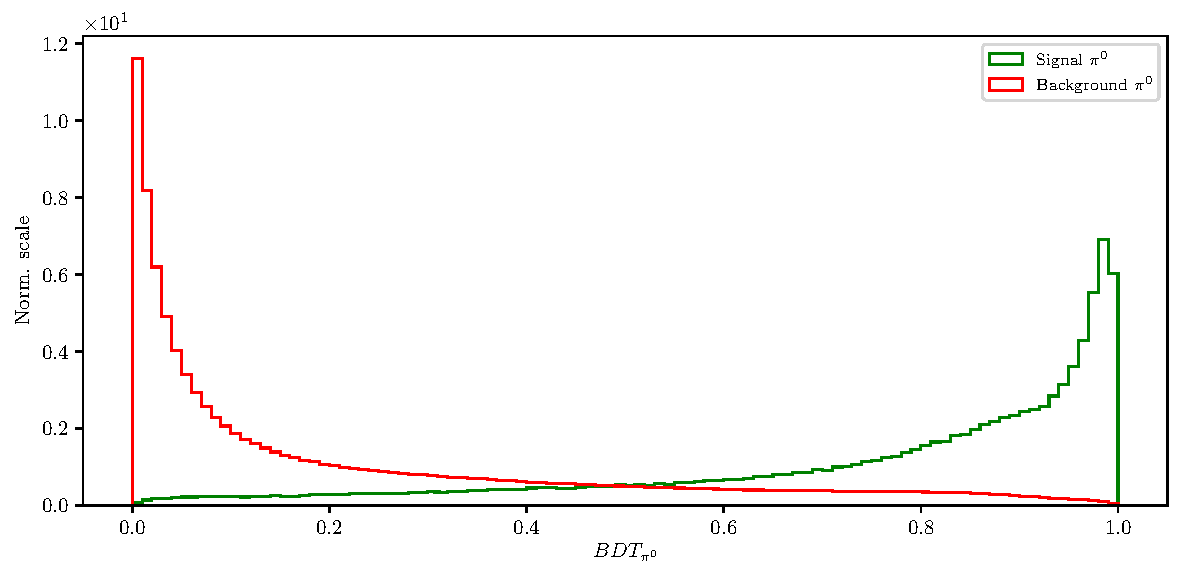
\includegraphics[width=\linewidth]{fig/ROECleanup_pi0}
	\caption{Classifier output of the $\pi^0$ training for signal and background $\pi^0$ candidates.}
	\label{fig:ROE_pi0}
\end{figure}

The distributions for all input variables and their correlations for signal and background candidates can be found in Appendix A for all steps of the ROE clean-up.


\subsection{\texorpdfstring{$\gamma$}{γ} MVA Training}

In this MVA training, we take the $\pi^0$ classifier output of the previous training as an input in order to train a classifier to distinguish between good and bad photons. The $\pi^0$ probability information from the previous step is applied to all photon pairs which pass the same $\pi^0$ selection criteria as defined in the previous step. Since it is possible to have overlapping pairs of photons, the $\pi^0$ probability is overwritten in the case of a larger value, since this points to a greater probability of a correct photon combination. On the other hand, some photon candidates fail to pass the $\pi^0$ selection, these candidates have a fixed value of $\pi^0$ probability equal to zero.

The training dataset of $\gamma$ candidates contains
\begin{itemize}
	\item 171699 target candidates,
	\item 177773 background candidates,
\end{itemize}
where the definition of a target is that the photon is an actual photon which is related to a primary MC particle. This tags all photon particles from secondary interactions as background photons. We use the converted $\gamma$ candidates from the existing Belle particle list. 

The input variables used in this MVA are
\begin{itemize}
	\item $p$ and $p_{CMS}$ of $\gamma$ candidates,
	\item $\pi^0$ probability,
	\item cluster quantities
	\begin{itemize}
		\item $E_9/E{25}$,
		\item theta angle,
		\item number of hit cells in the ECL,
		\item highest energy in cell,
		\item energy error,
		\item distance to closest track at ECL radius.
	\end{itemize}
\end{itemize}

The classifier output variable is shown in Figure \ref{fig:ROE_gamma}.

\begin{figure}[H]
	\centering
	\captionsetup{width=0.8\linewidth}
	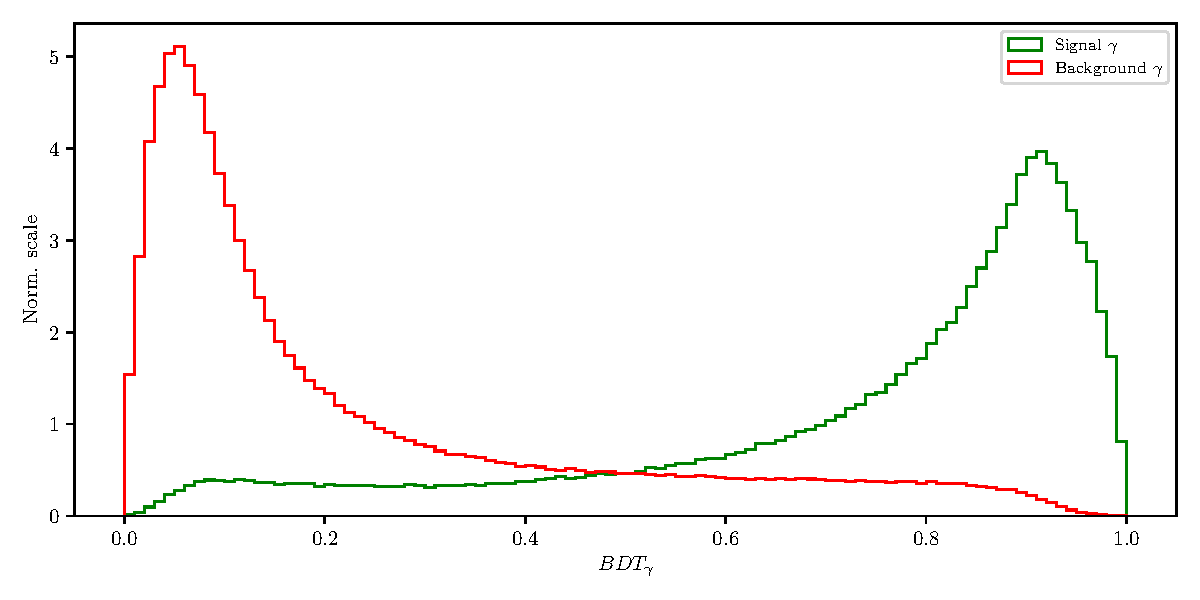
\includegraphics[width=\linewidth]{fig/ROECleanup_gamma}
	\caption{Classifier output of the $\gamma$ training for signal and background $\gamma$ candidates.}
	\label{fig:ROE_gamma}
\end{figure}

With the final weights for photon classification in hand, we apply them to the photon particle list. The selection optimization is shown in Figure \ref{fig:ROE_gamma_opt} (left), with the optimal selection on the $\gamma$ classifier output at
\begin{itemize}
	\item $BDT_\gamma > 0.5045$.
\end{itemize}

Figure \ref{fig:ROE_gamma_opt} (right) shows the LAB frame momentum of the photons in the logarithmic scale before and after the selection. The signal efficiency and background rejection of this clean-up step are
\begin{itemize}
	\item Signal efficiency: $\epsilon_{SIG} = 83.2~\%$,
	\item Background rejection: $1-\epsilon_{BKG} = 81.2~\%$.
\end{itemize}

\begin{figure}[H]
	\centering
	\captionsetup{width=0.8\linewidth}
	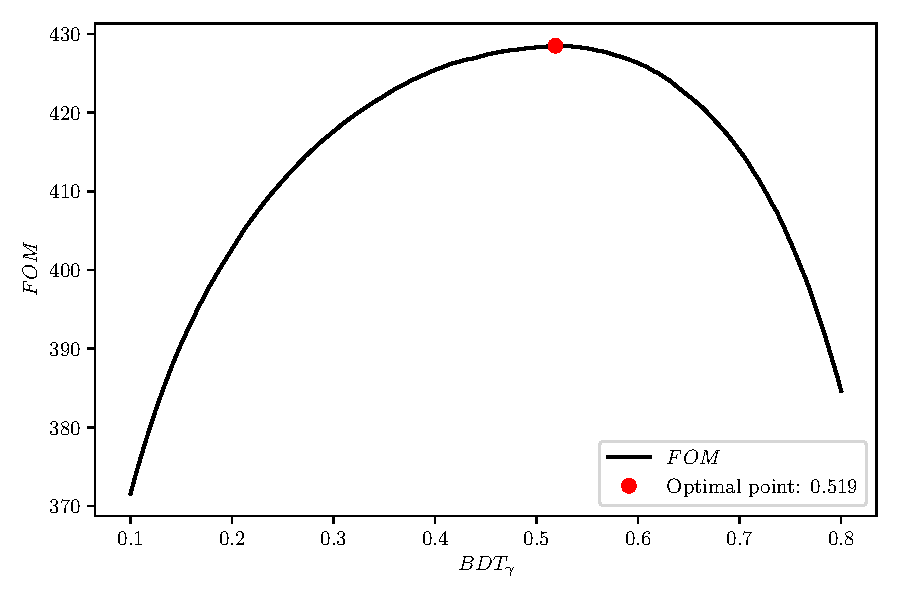
\includegraphics[width=\linewidth]{fig/ROECleanup_gamma_opt}
	\caption{The $\mathrm{FOM}$ of the classifier output optimization (left) and  momentum magnitude in the LAB frame (right) of signal and background photon candidates before (dashed) and after (solid) the optimal selection.}
	\label{fig:ROE_gamma_opt}
\end{figure}

The event is now considered to be clean of extra clusters.

\section{Tracks Clean-up}

Charged particles leave hits in the detector, which are then grouped into tracks by advanced tracking algorithms. The track is fitted and the track momentum is determined. With the help of particle identification information (PID), we are able to make an intelligent decision about the mass hypothesis of the particle and thus reconstruct the charged particle's four-momentum, which is then added in the loop in Eq. (\ref{eq:ROEloop}).

Most of the quality (good) tracks, which come from physics event of interest, come from the IP region, where the collisions occur. Cleaning up the tracks is a more complex procedure than cleaning up the clusters. The following facts need to be taken into account
\begin{enumerate}[(a)]
	\item good tracks can also originate away from the IP region, due to decays of long-lived particles, such as $K_S^0 \to \pi^+ \pi^-$,
	\item charged particles from background sources produce extra tracks or duplicates,
	\item low momentum charged particles can curl in the magnetic field and produce multiple tracks,
	\item secondary interactions with detector material or decays of particles in flight can produce "kinks" in the flight directory, resulting in multiple track fit results per track.
\end{enumerate}

Schematics of all the cases mentioned above are shown in Figure \ref{fig:track_cleanup}.

\begin{figure}[H]
	\centering
	\subfigure[]{
		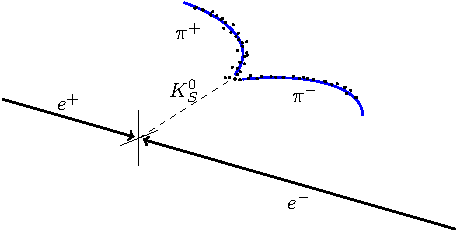
\includegraphics[width=0.49\linewidth]{texfig/V0}}%
	\subfigure[]{
		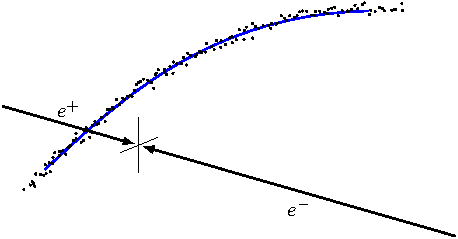
\includegraphics[width=0.49\linewidth]{texfig/background}}\\
	\subfigure[]{
		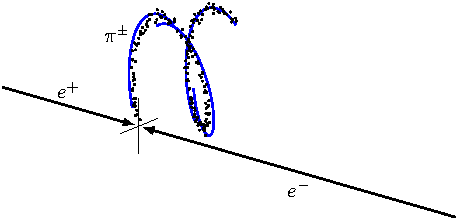
\includegraphics[width=0.49\linewidth]{texfig/curler}}%
	\subfigure[]{
		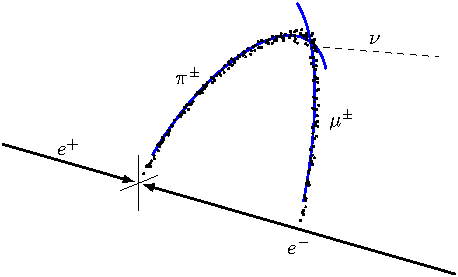
\includegraphics[width=0.49\linewidth]{texfig/decay}}%
	\captionsetup{width=.8\linewidth}
	\caption{(a) Tracks from long-lived neutral particles, which decay away from the IP region, (b) Random tracks from background which are reconstructed, (c) Low-momentum particles which curl in the magnetic field, (d) in-flight decays of particles, which produce a kink in the trajectory.}
	\label{fig:track_cleanup}
\end{figure}

It is obvious that tracks from the same momentum source should only be taken into account once, or, in the case of background tracks, not at all. Such tracks will from this point on be denoted as \textit{extra} tracks, because they add extra four-momentum to our final calculations in Eq. (\ref{eq:ROEloop}). At the same time, we have to take care that we do not identify \textit{good} tracks as \textit{extra} tracks. Both of these cases have negative impacts on the final resolution of all variables which depend on information from ROE.

\subsection{Tracks from Long-lived Particles}

The first step in tracks clean-up is taking care of tracks from long-lived particles, such as $K_S^0 \to \pi^+\pi^-$, $\gamma \to e^+ e^-$ and decays of $\Lambda$ baryons. Here we only focus on $K_S^0$, since they are the most abundant. This step is necessary because of the $\pi^\pm$ particles, coming from the $K_S^0$ decays, have large impact parameters, which is usually a trait of background particles. In order to minimize confusion from the MVA point-of-view, these tracks are taken into account separately.

We use the converted $K_S^0$ candidates from the existing Belle particle list and use a pre-trained Neural Network classifier in order to select only the good $K_S^0$ candidates. Figure \ref{fig:ROE_V0} shows the distribution of the $K_S^0$ invariant mass for signal and background candidates, before and after the selection cut on the classifier output. The momentum of selected $K_S^0$ candidates is added to the ROE, while the daughter tracks are discarded from our set.

\begin{figure}[H]
	\centering
	\captionsetup{width=0.8\linewidth}
	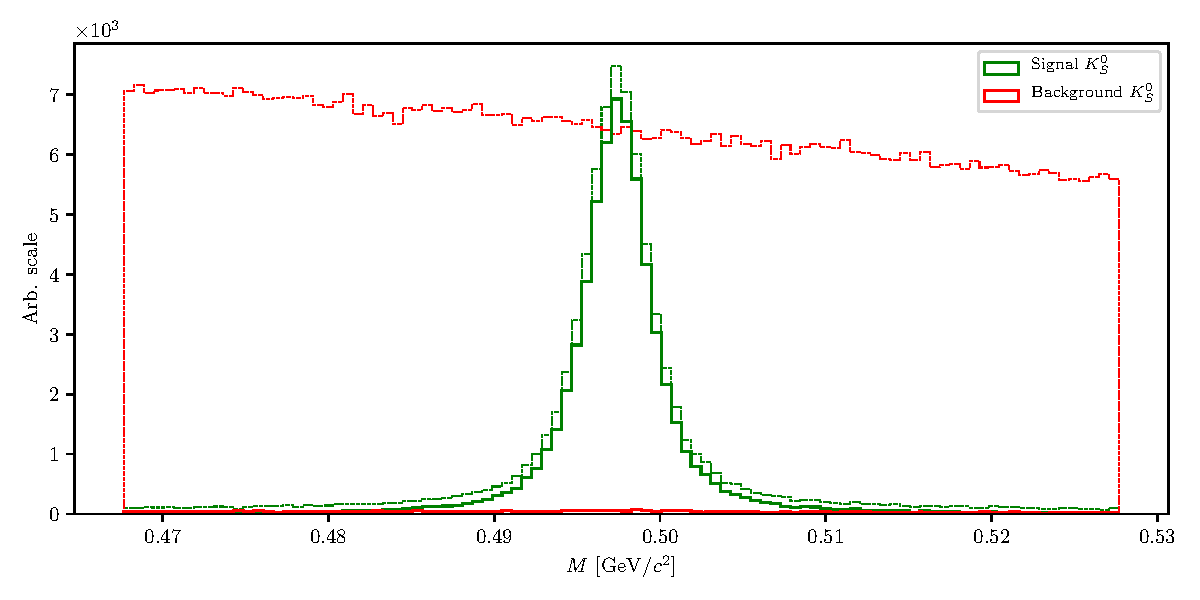
\includegraphics[width=\linewidth]{fig/ROECleanup_V0}
	\caption{Invariant mass of the $K_S^0$ candidates before (dashed) and after (solid) the selection on the Neural Network classifier for signal (green) and background candidates (red). Signal peaks at nominal $K_S^0$ mass, while background covers a wider region.}
	\label{fig:ROE_V0}
\end{figure}

The signal efficiency and background rejection for $K_S^0$ candidates after this selection and on the full range are
\begin{itemize}
	\item Signal efficiency: $\epsilon_{SIG} = 80.7~\%$,
	\item Background rejection: $1-\epsilon_{BKG} = 99.4~\%$.
\end{itemize}

\subsection{Duplicate Tracks}
All good tracks at this point should be coming from the IP region, since we took care of all the good tracks from long-lived particle decays, therefore we apply a selection on impact parameters for all the remaining tracks
\begin{itemize}
	\item $\vert d_0 \vert < 10\e{cm}$ and $\vert z_0 \vert < 20\e{cm}$
\end{itemize} 

and proceed with the clean-up of track duplicates.

\subsubsection{Defining a duplicate track pair}

In this step, we wish to find a handle on secondary tracks from low momentum curlers and decays in flight. The main property for these cases is that the 3D opening angle between such two tracks is very close to $0^\circ$ or $180^\circ$, since tracks deviate only slightly from the initial direction, but can also be reconstructed in the opposite way. Figure \ref{fig:ROE_dupAngleInit} shows the distribution of the angle between two tracks in a single pair for random track pairs and duplicate track pairs, where the latter were reconstructed as two same-sign or opposite-sign tracks.

\begin{figure}[H]
	\centering
	\captionsetup{width=0.8\linewidth}
	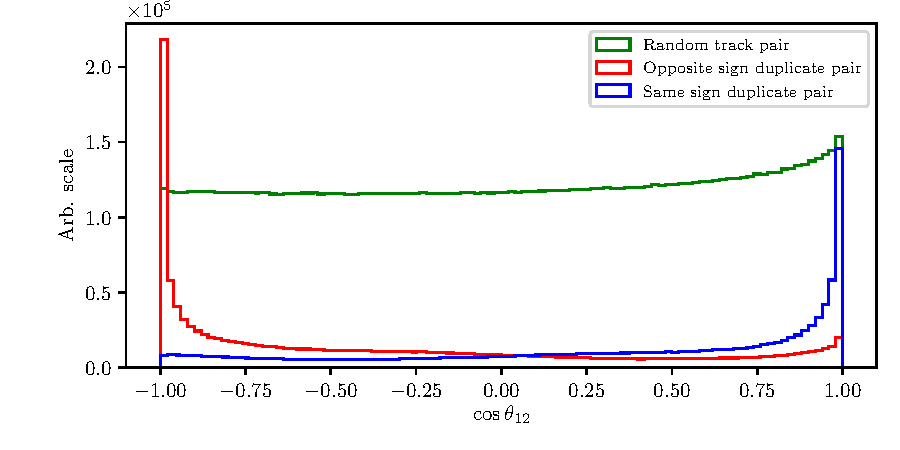
\includegraphics[width=\linewidth]{fig/ROECleanup_dup_angle_initial}
	\caption{Distribution of the angle between two tracks in a single pair for random track pairs (green) and duplicate track pairs, where the latter were reconstructed as two same-sign (blue) or opposite-sign tracks (red).}
	\label{fig:ROE_dupAngleInit}
\end{figure}

If the particle decayed mid-flight or produced multiple tracks due to being a low-momentum curler, then, as the name suggests, these particles most likely had low momentum in the transverse direction, $p_T$. Since both tracks originate from the same initial particle, the momentum difference should also peak at small values. Figure \ref{fig:ROE_dupPt} shows the momentum and momentum difference of tracks which belong to a random or a duplicate track pair.

\begin{figure}[H]
	\centering
	\captionsetup{width=0.8\linewidth}
	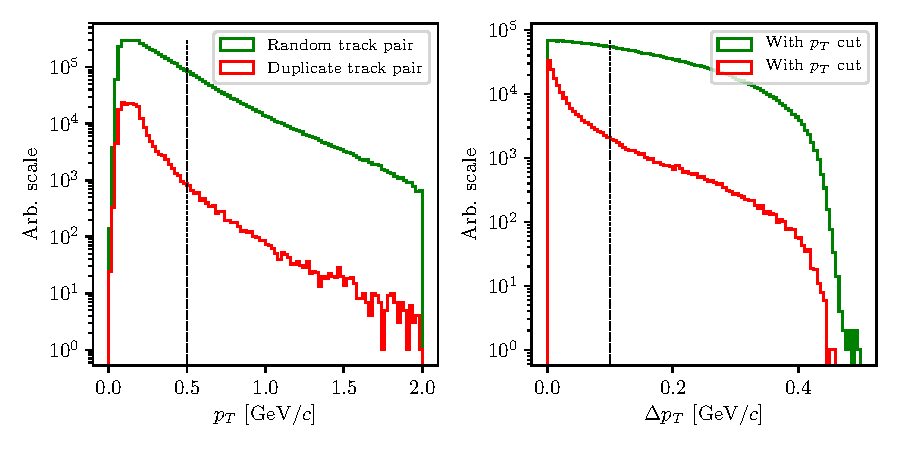
\includegraphics[width=\linewidth]{fig/ROECleanup_dup_pt}
	\caption{Distribution of transverse momentum $p_T$ (left) and transverse momentum difference $\Delta p_T$ (right) for all tracks coming from random (green) or duplicate track pairs (red). The plot on the right already includes the selection on $p_T$ from the plot on the left.}
	\label{fig:ROE_dupPt}
\end{figure}

We impose a selection of
\begin{itemize}
	\item $p_T < 0.5\e{GeV}/c$,
	\item $\vert \Delta p_T \vert < 0.1\e{GeV}/c$,
\end{itemize}

in order to minimize the number of random track pairs, while retaining a high percentage of duplicate track pairs. After applying all the selection criteria defined in this chapter, the final distribution of the angle between two tracks is shown in Figure \ref{fig:ROE_dupAngleFinal}.

\begin{figure}[H]
	\centering
	\captionsetup{width=0.8\linewidth}
	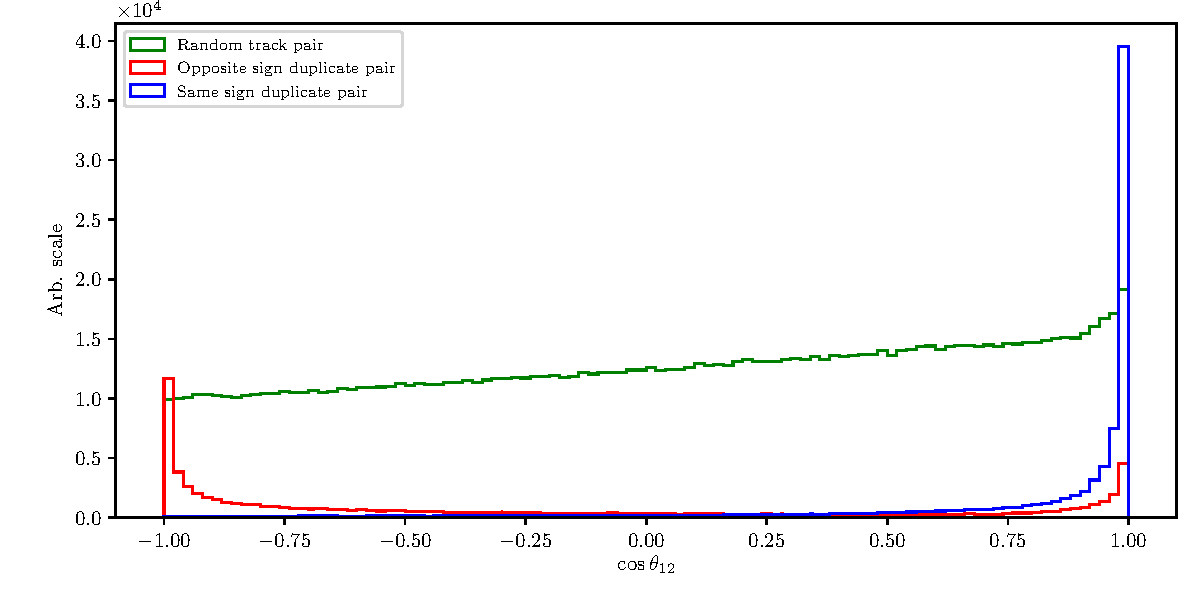
\includegraphics[width=\linewidth]{fig/ROECleanup_dup_angle_final}
	\caption{Distribution of the angle between two tracks in a single pair after applying the selection defined in this section. The distributions are shown for random track pairs (green) and duplicate track pairs, where the latter were reconstructed as two same-sign (blue) or opposite-sign tracks (red).}
	\label{fig:ROE_dupAngleFinal}
\end{figure}

\subsubsection{Training the duplicate track pair MVA}
\label{ss:trackMVA}

This final sample of track pairs is now fed into an MVA, which is trained to recognize duplicate track pairs over random ones. The training dataset contains
\begin{itemize}
	\item 113707 target candidates,
	\item 190314 background candidates,
\end{itemize}
where the definition of a target is that the track pair is a duplicate track pair. 

The input variables used in this MVA are
\begin{itemize}
	\item angle between tracks,
	\item track quantities
	\begin{itemize}
		\item impact parameters $d_0$ and $z_0$,
		\item transverse momentum $p_T$,
		\item helix parameters and helix parameter errors of the track,
		\item track fit $p$-value,
		\item number of hits in the SVD and CDC detectors
	\end{itemize}
\end{itemize}

The classifier is able to distinguish between random and duplicate track pairs in a very efficient manner, as shown in Figure \ref{fig:ROE_dupBDT}.

\begin{figure}[H]
	\centering
	\captionsetup{width=0.8\linewidth}
	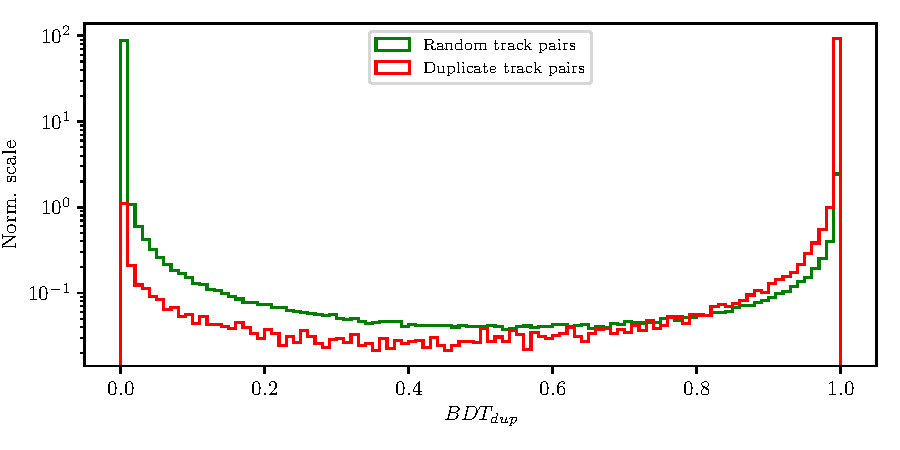
\includegraphics[width=\linewidth]{fig/ROECleanup_dup}
	\caption{Classifier output of the track pair training for random track pairs and duplicate track pairs.}
	\label{fig:ROE_dupBDT}
\end{figure}

The $\mathrm{FOM}$ function for optimal selection is shown in Figure \ref{fig:ROE_dupOpt} (left), along with the angle between the two tracks before and after the optimal selection (right). The optimal duplicate track selection is
\begin{itemize}
	\item $BDT_{duplicate} > 0.9985.$
\end{itemize}

The signal efficiency and background rejection for duplicate pair candidates after this selection is
\begin{itemize}
	\item Signal efficiency: $\epsilon_{SIG} = 87.2~\%$,
	\item Background rejection: $1-\epsilon_{BKG} = 98.8~\%$,
\end{itemize}
where signal and background represent duplicate and random track pairs, respectively.


\begin{figure}[H]
	\centering
	\captionsetup{width=0.8\linewidth}
	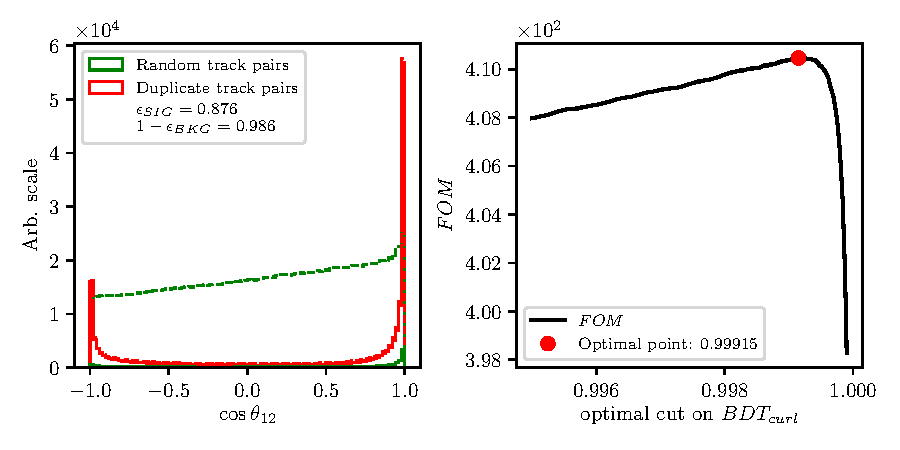
\includegraphics[width=\linewidth]{fig/ROECleanup_dup_opt}
	\caption{The optimization of the $\mathrm{FOM}$ function for the cut on classifier output (left) and distribution of the angle between two tracks in a single pair before (dashed) and after (solid) applying the optimal cut on the output classifier for random and duplicate track pairs (right).}
	\label{fig:ROE_dupOpt}
\end{figure}

\subsubsection{Defining duplicate tracks}

What remains now is to decide which track from the duplicate track pair to keep and which to discard. For this purpose, we apply duplicate pair-level information to each track in the pair in the form of
\begin{equation}
\Delta f = f_{this} - f_{other},
\end{equation}

where $f$ is an arbitrary variable from the list of track quantities in Section \ref{ss:trackMVA}. From the point-of-view of \textit{this} track, a track is more $duplicate$-like if the following is true
\begin{itemize}
	\item $\Delta d_0,\,\Delta z_0 > 0$ (\textit{this} track further away from the IP region),
	\item $\Delta p_T,\,\Delta p_Z < 0$ (\textit{this} track has lower momentum),
	\item $\Delta N_{SVD},\,\Delta N_{CDC} < 0$ (\textit{this} track has less hits in the SVD and CDC),
\end{itemize}

Additionally we define an MC truth variable 
\begin{equation}
\label{eq:chi2}
\Delta \chi^2 = \chi^2_{this} - \chi^2_{other},\quad\chi^2 = \sum_{i=x,y,z}\frac{\left(p_i - p_i^{MC}\right)^2}{\sigma(p_i)^2},
\end{equation}
where we compare all components of track momentum to the true values. If $\Delta \chi^2 > 0$, then \textit{this} track has a higher probability of being a duplicate track and should be discarded.

However, it turns out that solving this problem is not as simple as discarding one track and keeping the other one. An additional complication here is that we can have more than one extra track from the same initial particle, which leads to track pairs where both tracks are track duplicates. For example, if we have the following case
\begin{align*}
t_1&: \mathrm{good~track},\\
t_2&: \mathrm{extra~track},\\
t_3&: \mathrm{extra~track},\\
\mathrm{pair}_1&:\left(t_1,t_2\right),\\
\mathrm{pair}_2&:\left(t_1,t_3\right),\\
\mathrm{pair}_3&:\left(t_2,t_3\right),
\end{align*}
where $t_1$ is the original track and $t_2$ and $t_3$ are extra tracks, with $t_3$ being even more duplicate-like with respect to $t_2$. Here tracks $t_2$ and $t_3$ should be discarded while $t_1$ should be kept. We can achieve this if we overwrite existing pair-level information in the tracks for cases where the variable difference $\Delta f$ is more duplicate-like. If we follow the same example, we could fill information about the property $f$ in six different orders. 
\begin{align*}
1.&~\left(t_1,t_2*\right)\quad \to \quad \left(t_1,t_3*\right)\quad \to \quad \left(t_2*,t_3*\right),\\ 
2.&~\left(t_1,t_2*\right)\quad \to \quad \left(t_2*,t_3*\right)\quad \to \quad \left(t_1,t_3*\right),\\ 
3.&~\left(t_1,t_3*\right)\quad \to \quad \left(t_2,t_3*\right)\quad \to \quad \left(t_1,t_2*\right),\\
4.&~\left(t_1,t_3*\right)\quad \to \quad \left(t_1,t_2*\right)\quad \to \quad \left(t_2*,t_3*\right),\\
5.&~\left(t_2,t_3*\right)\quad \to \quad \left(t_1,t_3*\right)\quad \to \quad \left(t_1,t_2*\right),\\
6.&~\left(t_2,t_3*\right)\quad \to \quad \left(t_1,t_2*\right)\quad \to \quad \left(t_1,t_3*\right),
\end{align*}

where the "*" symbol denotes when a track is recognized as a duplicate track with respect to the other track. We see that no matter the order, both $t_2$ and $t_3$ get recognized as duplicate tracks correctly. %If you are a part of my defense committee and actually read this before my thesis defense, let me know, I owe you a bottle of whiskey.
%TODO: easter egg

\subsubsection{Training the duplicate track MVA}
The training procedure is similar as before. The sample of tracks from duplicate track pairs is now fed into an MVA, which is trained to distinguish duplicate tracks from good tracks. The training dataset contains
\begin{itemize}
	\item 84339 target candidates,
	\item 68280 background candidates,
\end{itemize}
where the definition of a target is that the track is a duplicate track. 

The input variables used in this MVA are
\begin{itemize}
	\item theta angle of the track momentum,
	\item track quantities
	\begin{itemize}
		\item impact parameters $d_0$ and $z_0$ and their errors,
		\item CMS frame momentum $p_{CMS}$ and momentum components $p_T$ and $p_z$ 
		\item number of hits in the SVD and CDC detectors
		\item track fit $p$-value,
	\end{itemize}
	\item pair-level information
	\begin{itemize}
		\item $\Delta d_0$, $\Delta z_0$, $\Delta N_{CDC}$, $\Delta N_{SVD}$, $\Delta p_T$, $\Delta p_z$, $\Delta p$-value.  
	\end{itemize}
\end{itemize}

The weights from this training are applied to the tracks, where now each track has a certain probability of being a duplicate track. We then compare these values between both tracks in each track pair as
\begin{equation}
\Delta BDT_{final} = BDT_{final}^{this} - BDT_{final}^{other},
\end{equation}
which is again applied to all track pairs and overwritten for tracks which are more duplicate-like. The classifier output and the classifier output difference for each track are shown in Figure \ref{fig:ROE_curl}. 

\begin{figure}[H]
	\centering
	\captionsetup{width=0.8\linewidth}
	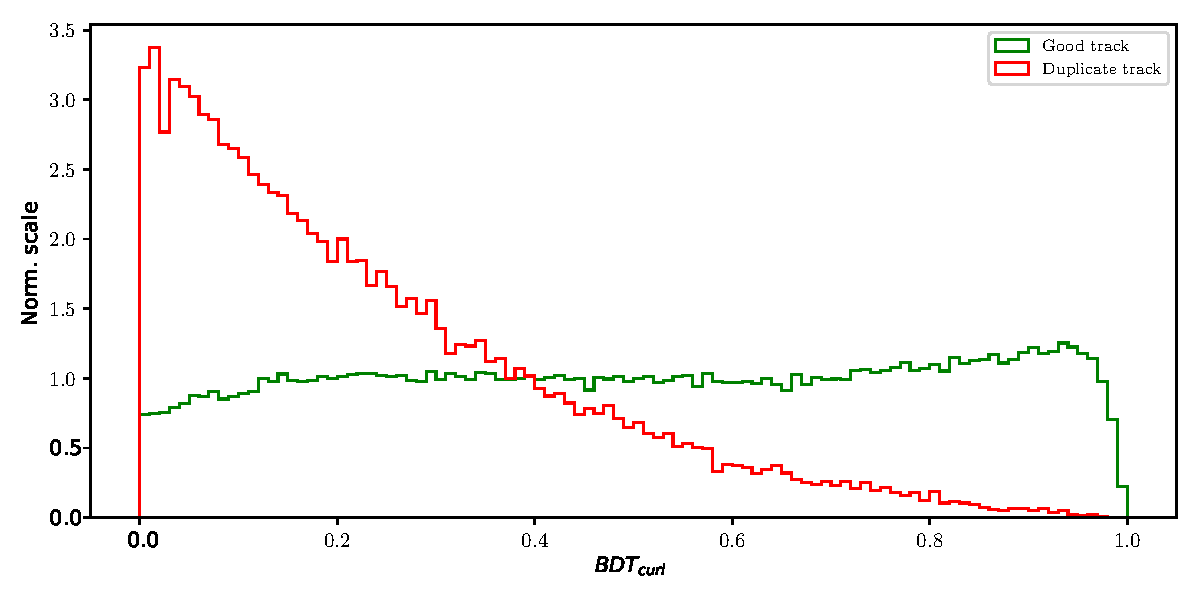
\includegraphics[width=\linewidth]{fig/ROECleanup_curl}
	\caption{Classifier output of the MVA training for curling track recognition (left) and difference of the classifier output, calculated for each track in a track pair (right).}
	\label{fig:ROE_curl}
\end{figure}

Finally, we select all duplicate tracks which survive the selection 
\begin{equation}
\Delta BDT_{final} > 0
\end{equation}

and discard them from our ROE. We can check the performance of our duplicate track classifier by applying the procedure to a validation sample of duplicate track pairs and compare the predicted result with the truth, based on Eq. (\ref{eq:chi2}). Table \ref{tab:rat} shows the performance of the duplicate track recognition in the form of percentages of correctly and incorrectly identified duplicate and original tracks. The model seems to perform well and the event is now considered to be clean of duplicate tracks.

\begin{table}[H]
	\centering
	\begin{tabular}{c|c|c}
		& Predicted duplicate track & Predicted good track \\
		\toprule
		Duplicate track & $83.07~\%$  & $22.62~\%$  \\
		Good track & $16.93~\%$ & $77.38\%$ \\
		\bottomrule
	\end{tabular}
	\captionsetup{width=.8\linewidth}
	\caption{Ratios of correctly classified and misclassified tracks.}
	\label{tab:rat}
\end{table}

\section{Belle Clean-up}

For comparison, we define the Belle clean-up, used standardly at Belle, which is much simpler and relies only on a set of basic selection criteria for neutral particles as well as charged ones. This clean-up procedure is not applied in addition to our ROE clean-up, but separately, only for comparison. 

In the case of photons, only a selection on the photon energy is applied, depending on the region where the photon hit the relevant part of the detector. The photon selection is summarized in Table \ref{tab:bellegamma}.

\begin{table}[H]
	\centering
	\begin{tabular}{c|c|c|c}
		& $17^\circ < \theta < 32^\circ$ & $32^\circ < \theta < 130^\circ$ & $130^\circ < \theta < 150^\circ$ \\
		\toprule
		$E_\gamma$ & $> 100\e{MeV}$  & $> 50\e{MeV}$ & $> 150\e{MeV}$  \\
		\bottomrule
	\end{tabular}
	\captionsetup{width=.8\linewidth}
	\caption{Photon selection for the Belle clean-up procedure. Different selection criteria are applied on photons in different parts of the detector.}
	\label{tab:bellegamma}
\end{table}

In case of tracks, pairs are selected which satisfy the following criteria:
\begin{itemize}
	\item $p_T < 275\e{MeV}/c$,
	\item $\Delta p = \vert \vec{p}_1 - \vec{p}_2\vert  < 100\e{MeV}/c$,
	\item $\cos \theta (\vec{p}_1,\vec{p}_2) < 15^\circ$ for same sign,
	\item $\cos\theta(\vec{p}_1,\vec{p}_2) > 165^\circ$ for opposite sign.
\end{itemize}

Of the two tracks, the one with a larger value of formula in Eq. \ref{eq:belleformula} is discarded. The remaining tracks in the event then need to satisfy the conditions described in Table \ref{tab:belletrack}.
\begin{equation}
\label{eq:belleformula}
\left(\gamma\vert d_0 \vert \right)^2 + \vert z_0 \vert^2, \quad \gamma = 5.
\end{equation}

\begin{table}[H]
	\centering
	\begin{tabular}{c|c|c|c}
		& $p_T < 250\e{MeV}/c$ & $250\e{MeV}/c < p_T < 500\e{MeV}/c$ & $p_T > 500\e{MeV}/c$ \\
		\toprule
		$\vert d_0 \vert$ & $< 20\e{cm}$  & $< 15\e{cm}$ & $< 10\e{cm}$  \\
		$\vert z_0 \vert$ & $< 100\e{cm}$  & $< 50\e{cm}$ & $< 20\e{cm}$  \\
		\bottomrule
		
	\end{tabular}
	\captionsetup{width=.8\linewidth}
	\caption{Photon selection for the Belle clean-up procedure. Different selection criteria are applied on photons in different parts of the detector}
	\label{tab:belletrack}
\end{table}

\section{Clean-up Results}

In this section, the results of the ROE clean-up are shown. It is obvious that cleaning up the event affects the shape of various distributions, especially \vars, which we are most interested in. Since the reconstruction procedure includes applying selection criteria on the cleaned-up variables, the clean-up also affects the efficiency of the reconstructed sample, not only the resolution. 

We compare the clean-up setup, defined in this analysis, to the standard clean-up used by Belle, and to a default case, where no clean-up was applied at all. We apply the clean-up procedure to our signal MC sample with all the applied selection criteria, defined in Section \ref{s:ss}, except for the signal categorization. Figure \ref{fig:roeopt} (left) shows signal candidate distributions of \vars~for various clean-up setups. Focusing on the ROE clean-up, we see an improvement in resolution in both observed variables and an overall decrease in efficiency. The efficiency decrease is expected since the cleaned-up variables are able to better isolate the perfectly reconstructed candidates and discard the non-perfect candidates. In fact, the efficiency of the perfectly reconstructed candidates increases after the ROE clean-up, as shown in Figure \ref{fig:roeopt} (right). The signal MC sample after in case of the Belle clean-up also shows a slight improvement in the resolution, but looking at the perfectly reconstructed candidates we see that this clean-up procedure is not optimal. Table \ref{tab:roeeff} shows ratios of efficiencies and $FWHM$'s of the clean-up procedures for the perfect signal with respect to the default case, based on the $\Delta E$ distribution. While both the Belle and ROE clean-up improve the resolution, ROE clean-up performs significantly better and also increases the amount of the perfectly reconstructed candidates in the final sample.

\begin{figure}[H]
	\centering
	\captionsetup{width=0.8\linewidth}
	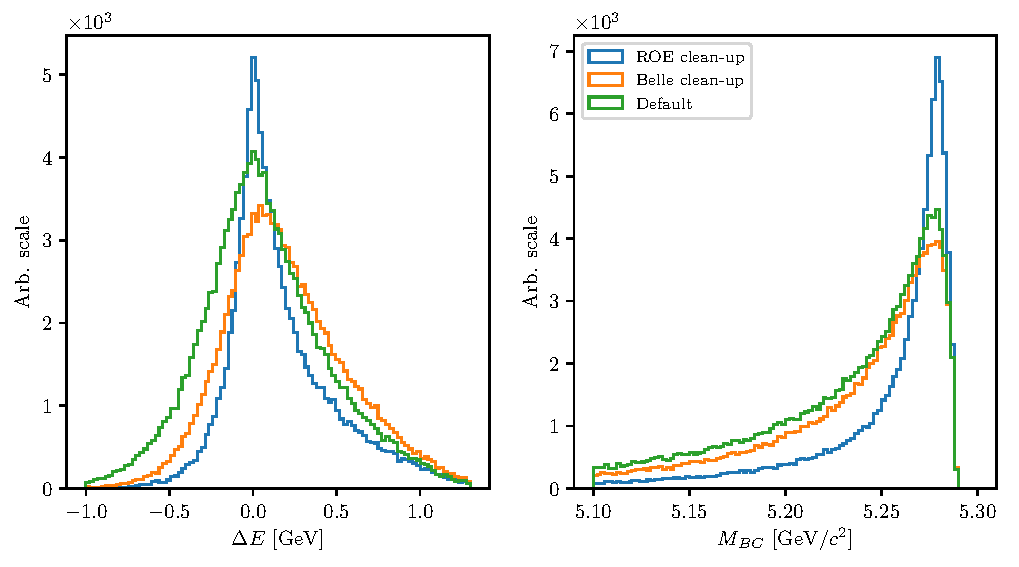
\includegraphics[width=\linewidth]{fig/roe_opt}
	\caption{\vars~distributions for various types of clean-up procedures. The figures on the left are shown for the full signal sample after the stated selection criteria, while the figures on the right are shown for the perfectly reconstructed signal candidates. For ROE clean-up, the procedure seems to improve resolution as well as increase the amount of perfectly reconstructed candidates, relative to the default case.}
	\label{fig:roeopt}
\end{figure}

\begin{table}[H]
	\centering
	\begin{tabular}{c|c|c}
		& Efficiency ratio & FWHM ratio \\
		\toprule
		Belle clean-up & $28.5~\%$  & $75.0~\%$  \\
		ROE clean-up & $140.1~\%$ & $35.0~\%$ \\
		\bottomrule
	\end{tabular}
	\captionsetup{width=.8\linewidth}
	\caption{Comparison of efficiencies and $FWHM$'s of ROE and Belle clean-up setups with respect to the default case (no clean-up).}
	\label{tab:roeeff}
\end{table}

Another variable which heavily depends on the clean-up is the charge product of the signal and companion $B$ meson candidate, already defined in Eq. (\ref{eq:chargeprod}), shown in Figure \ref{fig:roe_chargeproduct} for various clean-up procedures. The figure shows an improved resolution of the distribution, which means that candidates migrate to the correct value of the charge product after the clean-up. Looking at the perfectly reconstructed candidates we again see the increase in the bin corresponding to the correct charge product. As a cross-check, we can also look at \vars~variables for each value of the charge product. These plots are shown for the full signal MC sample in Figure \ref{fig:roe_split} and they show a clear resolution improvement for the correct value of the charge product in the case of the ROE clean-up. For other values of the charge product, there also seems to be a small improvement for both cases of clean-up, but it is negligible compared to the plots in the second column. This supports our choice of signal categorization, defined in Section \ref{sec:event-categorization}, where we select only candidates with the correct value of the charge product.

\begin{figure}[H]
	\centering
	\captionsetup{width=0.8\linewidth}
	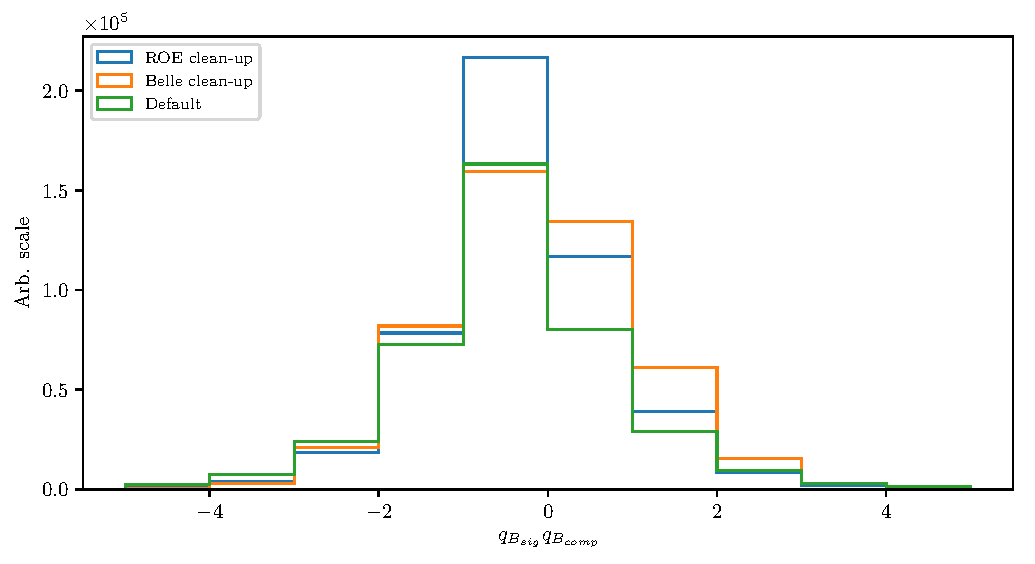
\includegraphics[width=\linewidth]{fig/roe_chargeprod}
	\caption{Distribution of the charge product of both $B$ mesons for various types of clean-up procedures, shown on the full signal MC (left) and for the perfectly reconstructed signal candidates (right). For ROE clean-up, the procedure seems to increase the number of perfectly reconstructed candidates.}
	\label{fig:roe_chargeproduct}
\end{figure}

\begin{figure}[H]
	\centering
	\captionsetup{width=0.8\linewidth}
	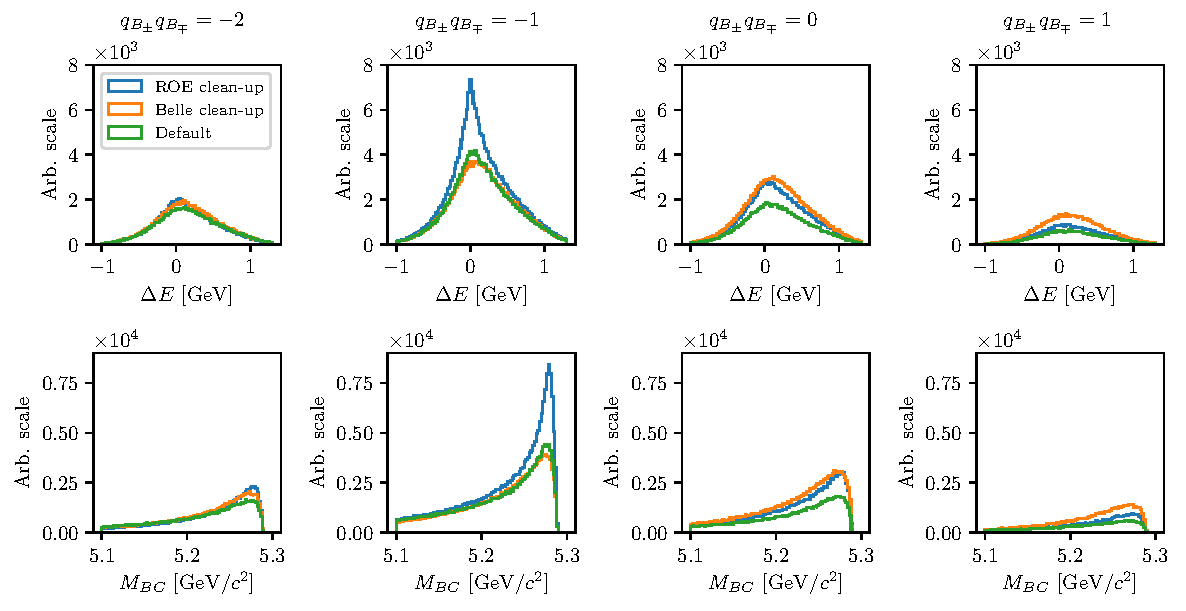
\includegraphics[width=\linewidth]{fig/roe_split}
	\caption{Distributions of $\Delta E$ (top) and $M_{BC}$ (bottom) for various types of clean-up procedures, split by specific values of the charge product, shown for the full signal MC. There is a significant improvement in resolution after ROE-cleanup for the case of the correct value of the charge product.}
	\label{fig:roe_split}
\end{figure}

\section{ROE Clean-up Validation}

The ROE clean-up seems to perform well on signal MC based on the results in the previous section. However, it is necessary to make sure that this procedure performs as well on other simulated and measured data, which is done in this section. The clean-up procedure is validated on the control sample, $$B^+ \to \bar D {}^0 \ell^+ \nu,\quad D^0 \to K^+K^-,$$
which was already defined in Section \ref{sec:control-decay}. The control candidates are reconstructed in the same manner as the signal candidates. In addition to the same selection criteria applied as in the previous section, we also apply a selection to make the control sample more significant. We keep only the candidates passing the following selection cut on the invariant mass of the two kaons
\begin{equation}
1.849\e{GeV}/c^2 < m_{KK} < 1.879\e{GeV}/c^2
\end{equation}
as shown in Figure \ref{fig:roe_mKK}.
\begin{figure}[H]
	\centering
	\captionsetup{width=0.8\linewidth}
	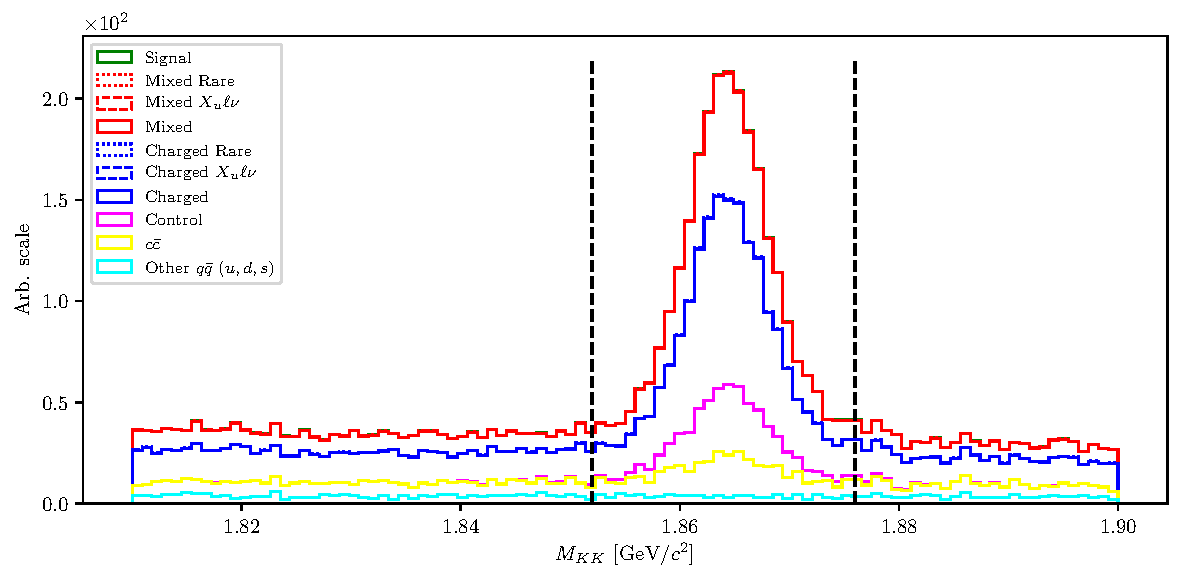
\includegraphics[width=\linewidth]{fig/roe_mKK_cut}
	\caption{Normalized distributions of $m_{KK}$ for the full MC dataset. The red lines represent the edges of the selection in the $m_{KK}$ distribution where the control sample is enhanced. The $m_KK$ distribution drops quickly for the case of the control decay, while staying uniform for other contributions.}
	\label{fig:roe_mKK}
\end{figure}

With the control sample selection determined, we now run the reconstruction with and without the ROE clean-up procedure on MC and data. For the purpose of this validation, we only run the reconstruction over 1 stream of the full available generated MC. 

The effects of the ROE clean-up are shown in Figure \ref{fig:roe_val}, where we overlay the data points to a stacked histogram of MC contributions for \vars. We see that data and MC agree well. A slight systematic trend can be seen in the $\Delta E$ variable, which is addressed in Section \ref{sec:smearing-and-offset-parameters}. The control sample resolution seems very poor in the case without the clean-up, but it improves significantly if the clean-up procedure is applied, as expected. The simulated background also seems to gain an improvement in the resolution, but this is likely due to the background consisting of similar candidates as the control sample. This means that the clean-up performs as expected due to the nature of the decays and does not arbitrarily shape the background to be more signal like. Additionally, it should be pointed out that, after the clean-up, the simulated background resolution is worse compared to the control decay resolution, while this is not the case if the clean-up procedure is not performed.
\begin{figure}[H]
	\centering
	\captionsetup{width=0.8\linewidth}
	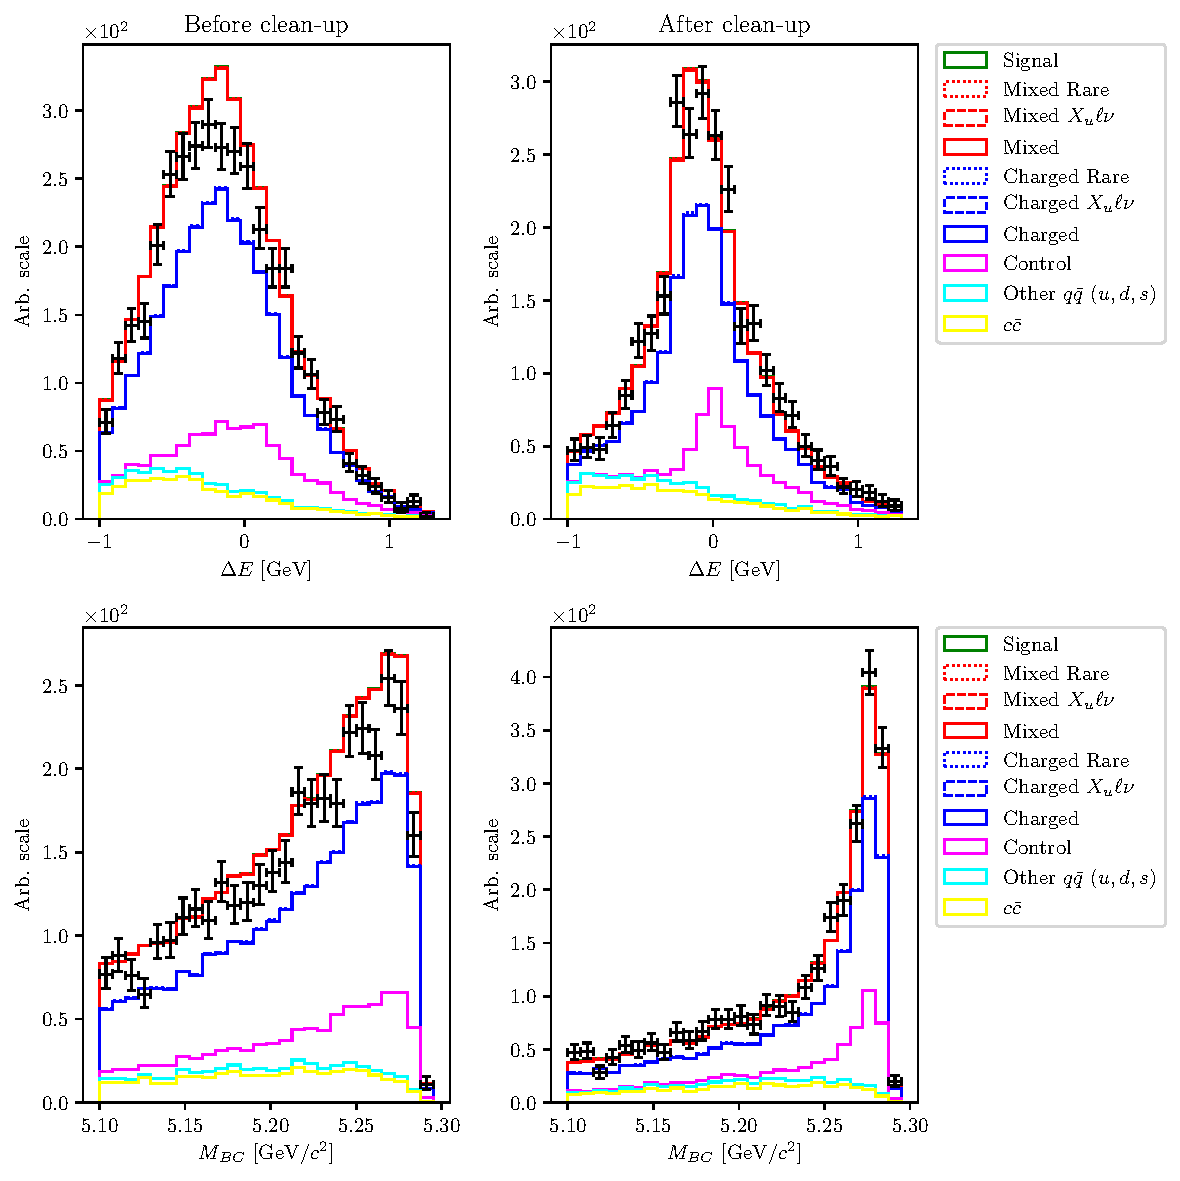
\includegraphics[width=\linewidth]{fig/roe_val}
	\caption{Distributions of $\Delta E$ (top) and $M_{BC}$ bottom for the case without (left) and with ROE clean-up (right). The resolution of the control sample is improved and the MC and data agree well in all aspects. While the simulated background resolution is also improved, it is worse compared to the resolution of the control sample.}
	\label{fig:roe_val}
\end{figure}

To perform the clean-up validation in greater detail we also compare the data and MC agreement in bins of the charge product of the two $B$ mesons. Figure \ref{fig:roe_val_split} shows the cleaned-up versions of \vars~for each charge product bin in the same manner as shown in the previous section. We see that the MC and data agreement persists in all cases. 
\begin{figure}[H]
	\centering
	\captionsetup{width=0.8\linewidth}
	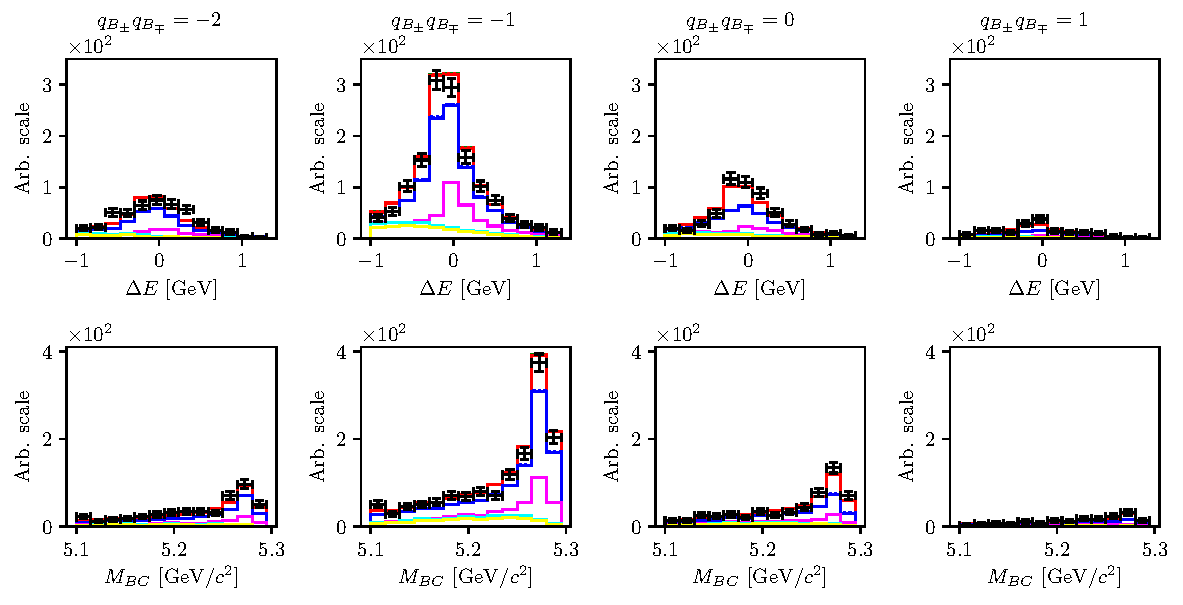
\includegraphics[width=\linewidth]{fig/roe_val_split}
	\caption{Distributions of $\Delta E$ (top) and $M_{BC}$ (bottom) split in bins of the charge product of the two $B$ mesons.}
	\label{fig:roe_val_split}
\end{figure}

The ROE clean-up procedure seems to perform well. It significantly improves the resolution of the signal/control candidates and increases the amount of perfectly clean events. The clean-up procedure was also applied to data and no disagreement with respect to the simulated MC samples was found. This means that the procedure does not differ between MC and data and does not affect them differently. The procedure was therefore validated in great detail and is suitable to be used in this analysis.